%iffalse
\let\negmedspace\undefined
\let\negthickspace\undefined
\documentclass[journal,12pt,onecolumn]{IEEEtran}
\usepackage[version=4]{mhchem}
\usepackage{chemformula} % for \ch if needed
\usepackage{chemfig}
\usepackage{chemmacros}
\chemsetup{modules = reactions} % Enables reaction arrows
\usepackage{graphicx}
\graphicspath{ {./images/} }
\usepackage{geometry}
\usepackage{lastpage}
\usepackage{cite}
\usepackage{amsmath,amssymb,amsfonts,amsthm}
\usepackage{enumitem,multicol}
\usepackage{algorithmic}
\usepackage{graphicx}
\usepackage{textcomp}
\usepackage{xcolor}
\usepackage{txfonts}
\usepackage{listings}
\usepackage{enumitem}
\usepackage{mathtools}
\usepackage{gensymb}
\usepackage{comment}
\usepackage[breaklinks=true]{hyperref}
\usepackage{tkz-euclide} 
\usepackage{listings}
\usepackage{gvv}                                        
%\def\inputGnumericTable{}                                 
\usepackage[latin1]{inputenc}                                
\usepackage{color}                                            
\usepackage{array}                                            
\usepackage{longtable}                                       
\usepackage{calc}                                             
\usepackage{multirow}                                         
\usepackage{hhline}                                           
\usepackage{ifthen}                                           
\usepackage{lscape}
\usepackage{tabularx}
\usepackage{array}
\usepackage{float}


\newtheorem{theorem}{Theorem}[section]
\newtheorem{problem}{Problem}
\newtheorem{proposition}{Proposition}[section]
\newtheorem{lemma}{Lemma}[section]
\newtheorem{corollary}[theorem]{Corollary}
\newtheorem{example}{Example}[section]
\newtheorem{definition}[problem]{Definition}
\newcommand{\BEQA}{\begin{eqnarray}}
\newcommand{\EEQA}{\end{eqnarray}}
\newcommand{\define}{\stackrel{\triangle}{=}}
\theoremstyle{remark}

\geometry{margin=1 in}



\setlength{\headheight}{14pt}
\setlength{\headsep}{5pt}
\setlength{\footskip}{20pt}
\begin{document}
1-5 carry one mark each 
\begin{enumerate}
  \item The fishermen, \rule{2cm}{0.15mm} the flood victims owed their lives, were rewarded by the government.

\hfill{GATE 2019 PI}

\begin{multicols}{2}
\begin{enumerate}
    \item whom
    \item to which
    \item to whom
    \item that
\end{enumerate}
\end{multicols}

\item Some students were not involved in the strike.

If the above statement is true, which of the following conclusions is/are logically necessary?

\begin{enumerate}[label=\arabic*.]
    \item Some who were involved in the strike were students.
    \item No student was involved in the strike.
    \item At least one student was involved in the strike.
    \item Some who were not involved in the strike were students.
\end{enumerate}

\hfill{GATE 2019 PI}

\begin{multicols}{2}
\begin{enumerate}
    \item 1 and 2
    \item 3
    \item 4
    \item 2 and 3
\end{enumerate}
\end{multicols}


\item The radius as well as the height of a circular cone increases by 10\%. The percentage increase in its volume is \rule{2cm}{0.15mm}.

\hfill{GATE 2019 PI}

\begin{multicols}{2}
\begin{enumerate}
    \item 17.1
    \item 21.0
    \item 33.1
    \item 72.8
\end{enumerate}
\end{multicols}

\item Five numbers 10, 7, 5, 4 and 2 are to be arranged in a sequence from left to right following the directions given below:
\begin{enumerate}
    \item No two odd or even numbers are next to each other.
    \item The second number from the left is exactly half of the left-most number.
    \item The middle number is exactly twice the right-most number.
\end{enumerate}
Which is the second number from the right?

\hfill{GATE 2019 PI}

\begin{multicols}{2}
\begin{enumerate}
    \item 2
    \item 4
    \item 7
    \item 10
\end{enumerate}
\end{multicols}
\item Until Iran came along, India had never been \rule{3cm}{0.15mm} in kabaddi.

\hfill{GATE 2019 PI}

\begin{multicols}{2}
\begin{enumerate}
    \item defeated
    \item defeating
    \item defeat
    \item defeatist
\end{enumerate}
\end{multicols}


6-10 carry two marks each
\item Since the last one year, after a 125 basis point reduction in repo rate by the Reserve Bank of India, banking institutions have been making a demand to reduce interest rates on small saving schemes. Finally, the government announced yesterday a reduction in interest rates on small saving schemes to bring them on par with fixed deposit interest rates.

Which one of the following statements can be inferred from the given passage?

\hfill{GATE 2019 PI}

\begin{multicols}{2}
\begin{enumerate}
    \item Whenever the Reserve Bank of India reduces the repo rate, the interest rates on small saving schemes are also reduced
    \item Interest rates on small saving schemes are always maintained on par with fixed deposit interest rates
    
    \item The government sometimes takes into consideration the demands of banking institutions before reducing the interest rates on small saving schemes
    \item A reduction in interest rates on small saving schemes follow only after a reduction in repo rate by the Reserve Bank of India
\end{enumerate}
\end{multicols}

\item In a country of 1400 million population, 70\% own mobile phones. Among the mobile phone owners, only 294 million access the Internet. Among these Internet users, only half buy goods from e-commerce portals. What is the percentage of these buyers in the country?

\hfill{GATE 2019 PI}

\begin{multicols}{2}
\begin{enumerate}
    \item 10.50
    \item 14.70
    \item 15.00
    \item 50.00
\end{enumerate}
\end{multicols}

\item The nomenclature of Hindustani music has changed over the centuries. Since the medieval period dhrupad styles were identified as baanis. Terms like gayaki and baaj were used to refer to vocal and instrumental styles, respectively. With the institutionalization of music education the term gharana became acceptable. Gharana originally referred to hereditary musicians from a particular lineage, including disciples and grand disciples.

Which one of the following pairings is NOT correct?

\hfill{GATE 2019 PI}

\begin{multicols}{2}
\begin{enumerate}
    \item dhrupad, baani
    \item gayaki, vocal
    \item baaj, institution
    \item gharana, lineage
\end{enumerate}
\end{multicols}
\item Two trains started at 7AM from the same point. The first train travelled north at a speed of 80 km/h and the second train travelled south at a speed of 100 km/h. The time at which they were 540 km apart is \rule{2cm}{0.15mm} AM.

\hfill{GATE 2019 PI}

\begin{multicols}{2}
\begin{enumerate}
    \item 9
    \item 10
    \item 11
    \item 11.30
\end{enumerate}
\end{multicols}

\item ``I read somewhere that in ancient times the prestige of a kingdom depended upon the number of taxes that it was able to levy on its people. It was very much like the prestige of a head-hunter in his own community.''

Based on the paragraph above, the prestige of a head-hunter depended upon \rule{3cm}{0.15mm}

\hfill{GATE 2019 PI}

\begin{multicols}{2}
\begin{enumerate}
    \item the prestige of the kingdom
    \item the prestige of the heads
    \item the number of taxes he could levy
    \item the number of heads he could gather
\end{enumerate}
\end{multicols}

\end{enumerate}




1-25 carry one mark each
\begin{enumerate}
 \item Let $r$ and $\theta$ be the modulus and argument of the complex number $z = 1 + i$, respectively. Then $(r, \theta)$ equals

\hfill{GATE 2019 PI}

\begin{multicols}{2}
\begin{enumerate}
    \item $(\sqrt{2}, \frac{\pi}{4})$
    \item $(2, \frac{\pi}{2})$
    \item $(2, \frac{\pi}{3})$
    \item $(\sqrt{2}, \pi)$
\end{enumerate}
\end{multicols}

\item Let $\lambda_1$ and $\lambda_2$ be the two eigenvalues of the matrix $A = \begin{pmatrix} 0 & -1 \\ 1 & 1 \end{pmatrix}$. Then, $\lambda_1 + \lambda_2$ and $\lambda_1 \lambda_2$, are respectively

\hfill{GATE 2019 PI}

\begin{multicols}{2}
\begin{enumerate}
    \item $1$ and $1$
    \item $1$ and $-1$
    \item $-1$ and $1$
    \item $-1$ and $-1$
\end{enumerate}
\end{multicols}

\item The Laplace transform of the function $f(t) = e^{-t}$ is given by

\hfill{GATE 2019 PI}

\begin{multicols}{2}
\begin{enumerate}
    \item $\dfrac{1}{(s+1)^2}$
    \item $\dfrac{1}{s-1}$
    \item $\dfrac{1}{s+1}$
    \item $\dfrac{1}{(s-1)^2}$
\end{enumerate}
\end{multicols}

\item The relative decline rate of oil is given by $\frac{1}{q} \frac{dq}{dt} = -aq^b$, where $q$ is the oil production rate, $a\;(>0)$ is the decline rate and $b$ is a constant. The equation gives harmonic decline curve when $b$ is

\hfill{GATE 2019 PI}

\begin{multicols}{2}
\begin{enumerate}
    \item 1.5
    \item 1
    \item 0.5
    \item 0
\end{enumerate}
\end{multicols}

\item Which one of the following provides a vertical stab for the flow lines and annulus access lines from multiple wells in offshore subsea completion?

\hfill{GATE 2019 PI}

\begin{multicols}{2}
\begin{enumerate}
    \item Moon pool deck
    \item Spider beams
    \item Telescopic joints
    \item Manifold
\end{enumerate}
\end{multicols}

\item In a faulted reservoir, the principle of superposition for the pressure drop using diffusivity equation is applicable. This is due to

\hfill{GATE 2019 PI}

\begin{multicols}{2}
\begin{enumerate}
    \item high Reynolds number flow in the well.
    \item constant permeability.
    \item pressure dependent viscosity.
    \item linearity of the diffusivity equation.
\end{enumerate}
\end{multicols}

\item Which one of the following parameters is measured using routine core analysis (RCA)?

\hfill{GATE 2019 PI}

\begin{multicols}{2}
\begin{enumerate}
    \item Porosity
    \item Relative permeability
    \item Capillary pressure
    \item Wettability
\end{enumerate}
\end{multicols}
\item Match the following:

\begin{tabular}{ll}
P.\ Induction Log         & I.\ Equivalent water resistivity \\
Q.\ Dielectric Log        & II.\ Resistivity \\
R.\ Self-Potential Log    & III.\ Conductivity \\
S.\ Electrical Log        & IV.\ Permittivity \\
\end{tabular}

\hfill{GATE 2019 PI}

\begin{multicols}{2}
\begin{enumerate}
    \item P-II, Q-IV, R-III, S-I
    \item P-III, Q-I, R-IV, S-II
    \item P-III, Q-II, R-IV, S-I
    \item P-III, Q-IV, R-I, S-II
\end{enumerate}
\end{multicols}

\item Which one of the following rocks and reservoir fluids are arranged in the decreasing order of their electrical resistivity? Assume that rocks have equal porosity and are filled with brine.

\hfill{GATE 2019 PI}

\begin{multicols}{2}
\begin{enumerate}
    \item Shale $>$ Brine $>$ Sandstone $>$ Limestone $>$ Gas
    \item Gas $>$ Shale $>$ Sandstone $>$ Limestone $>$ Brine
    \item Gas $>$ Limestone $>$ Sandstone $>$ Shale $>$ Brine
    \item Shale $>$ Brine $>$ Limestone $>$ Sandstone $>$ Gas
\end{enumerate}
\end{multicols}

\item Which one of the following is the correct sequence of events for hydrocarbon generation in the subsurface?

\hfill{GATE 2019 PI}

\begin{multicols}{2}
\begin{enumerate}
    \item Catagenesis $\rightarrow$ Metagenesis $\rightarrow$ Diagenesis
    \item Catagenesis $\rightarrow$ Diagenesis $\rightarrow$ Metagenesis
    \item Diagenesis $\rightarrow$ Catagenesis $\rightarrow$ Metagenesis
    \item Diagenesis $\rightarrow$ Metagenesis $\rightarrow$ Catagenesis
\end{enumerate}
\end{multicols}

\item Match the following:

\begin{tabular}{ll}
P.\ Bingham plastic               & I.\ $\tau = ky^n$ \\
Q.\ Power law                     & II.\ $\tau = \tau_y + ky^n$ \\
R.\ Power law with yield stress   & III.\ $\tau = \tau_y + \mu_p y$ \\
\end{tabular}

Here

\begin{tabular}{ll}
$\tau$ : & shear stress \\
$\tau_y$ : & yield value or yield stress \\
$\mu_p$ : & shear viscosity \\
$n$ : & power law index \\
$k$ : & consistency index \\
$\gamma$ : & shear rate \\
\end{tabular}

\hfill{GATE 2019 PI}

\begin{multicols}{2}
\begin{enumerate}
    \item P-II, Q-I, R-III
    \item P-I, Q-III, R-II
    \item P-III, Q-II, R-I
    \item P-III, Q-I, R-II
\end{enumerate}
\end{multicols}
\item Match the following for drill pipe failure:

\begin{tabular}{ll}
P.\ Twist off  & I.\ due to excessive tension \\
Q.\ Parting    & II.\ due to excessive torque \\
R.\ Collapse   & III.\ due to cyclic loading \\
S.\ Fatigue    & IV.\ due to extensive external pressure \\
\end{tabular}

\hfill{GATE 2019 PI}

\begin{multicols}{2}
\begin{enumerate}
    \item P-III, Q-IV, R-I, S-II
    \item P-II, Q-I, R-IV, S-III
    \item P-I, Q-II, R-III, S-IV
    \item P-IV, Q-III, R-II, S-I
\end{enumerate}
\end{multicols}

\item Which one of the following flow regimes is more favorable for gas lift operation?

\hfill{GATE 2019 PI}

\begin{multicols}{2}
\begin{enumerate}
    \item Bubbly flow
    \item Annular flow
    \item Churn flow
    \item Stratified flow
\end{enumerate}
\end{multicols}

\item H$_2$S gas is

\hfill{GATE 2019 PI}

\begin{multicols}{2}
\begin{enumerate}
    \item acidic.
    \item non-corrosive.
    \item lighter than air.
    \item non-flammable.
\end{enumerate}
\end{multicols}

\item Which one of the following offshore platforms \textbf{DOES NOT} use buoyant columns or pontoons?

\hfill{GATE 2019 PI}

\begin{multicols}{2}
\begin{enumerate}
    \item Tension leg platforms
    \item Jack up platforms
    \item Spar platforms
    \item Semi-submersible platforms
\end{enumerate}
\end{multicols}

\item In which one of the following offshore platforms, the condition of the sea floor is a vital consideration?

\hfill{GATE 2019 PI}

\begin{multicols}{2}
\begin{enumerate}
    \item Drill ship platforms
    \item Tension leg platforms
    \item Concrete gravity platforms
    \item Floating, production, storage and offloading (FPSO) platforms
\end{enumerate}
\end{multicols}

\item The `Klinkenberg effect' is related to

\hfill{GATE 2019 PI}

\begin{multicols}{2}
\begin{enumerate}
    \item viscous fingering during water flooding in oil reservoirs.
    \item hysteresis effect in relative permeability during drainage and imbibition process.
    \item oil viscosity dependence on temperature.
    \item slippage of gas phase at the sand grain surface.
\end{enumerate}
\end{multicols}

\item Favourable conditions for formation of gas hydrates are

\hfill{GATE 2019 PI}

\begin{multicols}{2}
\begin{enumerate}
    \item high temperature and high pressure.
    \item high temperature and low pressure.
    \item low temperature and high pressure.
    \item low temperature and low pressure.
\end{enumerate}
\end{multicols}
\item Match the following quantities with their dimensions:

\begin{tabular}{ll}
P.\ Viscosity        & I.\ $\mathrm{M^1\ L^{-1}\ T^{-2}}$ \\
Q.\ Permeability     & II.\ $\mathrm{M^0\ L^2\ T^0}$ \\
R.\ Compressibility  & III.\ $\mathrm{M^1\ L^{-1}\ T^{-1}}$ \\
S.\ Pressure         & IV.\ $\mathrm{M^{-1}\ L^{1}\ T^{2}}$ \\
\end{tabular}

\hfill{GATE 2019 PI}

\begin{multicols}{2}
\begin{enumerate}
    \item P-III, Q-II, R-IV, S-I
    \item P-II, Q-I, R-IV, S-III
    \item P-III, Q-I, R-IV, S-II
    \item P-I, Q-II, R-III, S-IV
\end{enumerate}
\end{multicols}
\item The plot of dissolved gas oil ratio ($R_s$), defined as the ``ratio of STP volume of gas dissolved in the oil at pressure $P$, to the volume of the oil at STP'' is given below.
\begin{figure}[H]
    \centering
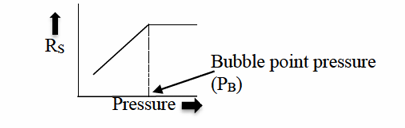
\includegraphics[width=0.5\linewidth]{figs/Q.20.png}
    \caption{}
    \label{fig:figs/Q.20.png}
\end{figure}
For the same oil, the plot of produced gas oil ratio ($R_P$) defined as the ``ratio of STP volume of the gas liberated from the oil at pressure $P$, to the volume of the oil at STP'' is
\hfill{GATE 2019 PI}
\begin{figure}[H]
    \centering
    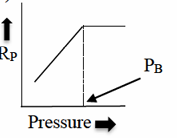
\includegraphics[width=1\linewidth]{Q.20.1.png}
    \caption{fig2}
    \label{fig:Q.20.1.png}
\end{figure}
\item Which one of the following denotes a regular four-spot flood pattern?


$\triangle$ represents injection well

$\circ$ represents production well
\begin{figure}[H]
    \centering
    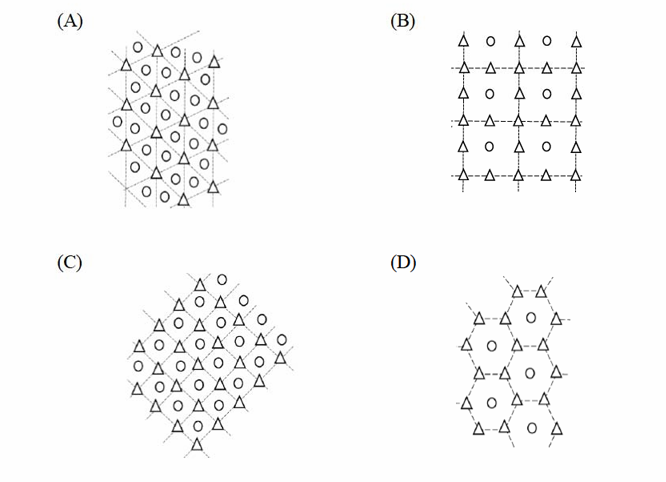
\includegraphics[width=1\linewidth]{figs/Q.21.png}
    \caption{fig3}
    \label{fig:figs/Q.21.png}
\end{figure}
\item The value of $\displaystyle \lim_{x \to 0} \frac{(x+1)\sin{x}}{x^2 + 2x}$ is \rule{3cm}{0.15mm} (round off to 2 decimal places).

\hfill{GATE 2019 PI}

\item Let $A = \begin{pmatrix} 1 & 2 \\ 2 & 1 \end{pmatrix}$, $X = \begin{pmatrix} 1 \\ b \end{pmatrix} a$, and $Y = \begin{pmatrix} 3 \\ 3 \end{pmatrix} \frac{1}{2}$. If $AX = Y$, then $a + b$ equals \rule{3cm}{0.15mm}.

\hfill{GATE 2019 PI}

\item Let $\vec{u} = i + j + a k$ and $\vec{v} = a^2 i + 4j - 4k$, where $i, j$ and $k$ are cartesian unit vectors. If $\vec{u}$ is perpendicular to $\vec{v}$, then $a$ equals \rule{3cm}{0.15mm}.

\hfill{GATE 2019 PI}

\item If the neutron log porosity ($\phi_N$) is 0.09 and density log porosity ($\phi_D$) is 0.24 in the cross-over region, then the average porosity of the gas bearing region is \rule{3cm}{0.15mm} (round off to 2 decimal places).

\hfill{GATE 2019 PI}



26-55 carry two marks each
\item The general solution of the differential equation $\dfrac{d^2 y}{dx^2} - 2\dfrac{dy}{dx} + y = 0$ is (here $C_1$ and $C_2$ are arbitrary constants)

\hfill{GATE 2019 PI}

\begin{multicols}{2}
\begin{enumerate}
    \item $y = C_1 e^{x} + C_2 e^{-x}$
    \item $y = C_1 x e^{x} + C_2 x e^{2x}$
    \item $y = C_1 e^{x} + C_2 x e^{-x}$
    \item $y = C_1 e^{x} + C_2 x e^{x}$
\end{enumerate}
\end{multicols}

\item Consider the following system of linear equations (where $p$ and $q$ are constants):

\[
\begin{aligned}
x_1 + x_2 + x_3 & = 1 \\
x_1 - x_2 + 2x_3 & = p \\
3x_1 - x_2 + 5x_3 & = q
\end{aligned}
\]

This system has at least one solution for any $p$ and $q$ satisfying

\hfill{GATE 2019 PI}

\begin{multicols}{2}
\begin{enumerate}
    \item $2p - q + 1 = 0$
    \item $2q + p + 1 = 0$
    \item $2p + q - 1 = 0$
    \item $2q + p - 1 = 0$
\end{enumerate}
\end{multicols}
\item Three reservoirs P, Q and R have identical geometry and rock properties. The plot of the height of the transition zone ($h$) above the free water level (FWL) against the water saturation ($S_w$) is given in the figure. Assume $\sigma \cos \theta$ for all the three fluid combinations remains the same. Which one of the following is the correct match of the reservoir fluids with the reservoir ($\sigma$ is the interfacial tension between the respective fluid phases and $\theta$ is the contact angle).
\begin{figure}[H]
    \centering
    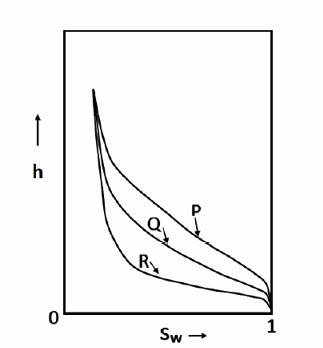
\includegraphics[width=0.5\linewidth]{figs/Q.28.png}
    \caption{fig4}
    \label{fig:figs/Q.28.png}
    
\end{figure}

\hfill{GATE 2019 PI}

\begin{multicols}{2}
\begin{enumerate}
    \item P: low density oil -- water,\quad Q: gas -- water,\quad R: high density oil -- water
    \item P: gas -- water,\quad Q: low density oil -- water,\quad R: high density oil -- water
    \item P: high density oil -- water,\quad Q: low density oil -- water,\quad R: gas -- water
    \item P: gas -- water,\quad Q: high density oil -- water,\quad R: low density oil -- water
\end{enumerate}
\end{multicols}
\item The fractional flow ($f_w$) versus water saturation ($S_w$) curve for an imbibition process (neglecting the capillary forces) in a given core for three different inclinations is shown in the figure.
\begin{figure}[H]
    \centering
    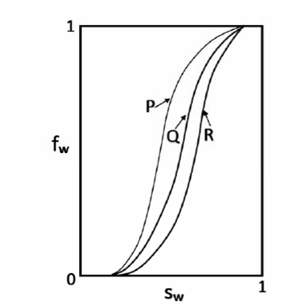
\includegraphics[width=0.5\linewidth]{figs/Q.29.png}
    \caption{fig5}
    \label{fig:figs/Q.29.png}
\end{figure}
Which one of the following is the correct representation of the fractional flow curevs?
\hfill{GATE 2019 PI}

\begin{multicols}{2}
\begin{enumerate}
    \item P: Down-dip, \quad Q: No-dip, \quad R: Up-dip
    \item P: Down-dip, \quad Q: Up-dip, \quad R: No-dip
    \item P: No-dip, \quad Q: Down-dip, \quad R: Up-dip
    \item P: Up-dip, \quad Q: No-dip, \quad R: Down-dip
\end{enumerate}
\end{multicols}


\item Match the following:

\begin{tabular}{ll}
P. Dynamic positioning        & I.\ Self-contained drilling rig on a floating barge, fitted with long support legs that can be raised or lowered independently of each other. \\
Q. Mooring                   & II.\ A system which automatically controls a vessel's position and heading exclusively by means of active thrust. \\
R. Jack-up                   & III.\ Remains afloat by weight and buoyancy balance. \\
S. Semi-submersible platform & IV.\ A system that is used for station keeping of a floating platform or ship at any depth. \\
\end{tabular}

\hfill{GATE 2019 PI}

\begin{multicols}{2}
\begin{enumerate}
    \item P-IV, Q-II, R-I, S-III
    \item P-III, Q-I, R-IV, S-II
    \item P-II, Q-IV, R-I, S-III
    \item P-II, Q-IV, R-III, S-I
\end{enumerate}
\end{multicols}
\item Match the following:

\begin{center}
\begin{tabular}{|p{0.52\textwidth}|p{0.38\textwidth}|}
\hline
P. Increase in sweep efficiency at the macroscopic-level by increasing water viscosity & I. LPG injection \\
\hline
Q. Increase in sweep efficiency at the macroscopic-level by decreasing oil viscosity & II. Surfactant flooding \\
\hline
R. Increase in displacement efficiency at the pore-scale by using a miscible displacing fluid & III. In-situ combustion \\
\hline
S. Increase in displacement efficiency at the pore-scale by reducing interfacial tension & IV. Polymer flooding \\
\hline
\end{tabular}
\end{center}

\hfill{GATE 2019 PI}

\begin{multicols}{2}
\begin{enumerate}
    \item P-I, Q-IV, R-III, S-II
    \item P-I, Q-II, R-IV, S-III
    \item P-IV, Q-III, R-I, S-II
    \item P-IV, Q-I, R-II, S-III
\end{enumerate}
\end{multicols}
\item An exploratory well encountered three reservoir formations S1 (perfectly cemented), S2 (poorly cemented) and S3 (fractured). The Formation Factor ($F$) is governed by the equation $F = a\phi^{-m}$, where `$\phi$' is the porosity and `$m$' is the cementation factor. The constant `$a$', linked to tortuosity is assumed to be 1 for all the formations. The log-log plot between Formation Factor ($F$) and porosity ($\phi$) is shown.
\begin{figure}[H]
    \centering
    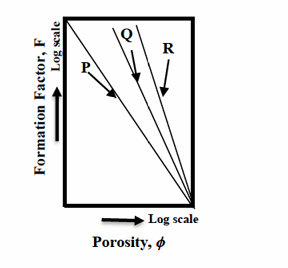
\includegraphics[width=0.5\linewidth]{figs/Q.32.png}
    \caption{fig6}
    \label{fig:figs/Q.32.png}
\end{figure}
\hfill{GATE 2019 PI}

\begin{multicols}{2}
\begin{enumerate}
    \item S1-P, S2-Q, S3-R
    \item S1-R, S2-P, S3-Q
    \item S1-P, S2-R, S3-Q
    \item S1-R, S2-Q, S3-P
\end{enumerate}
\end{multicols}
\item Typical parameters obtained in the pyrolysis experiment of the source rock materials are shown in the Figure. Which one of the following is NOT true about pyrolysis in source rock analysis?
\begin{figure}[H]
    \centering
    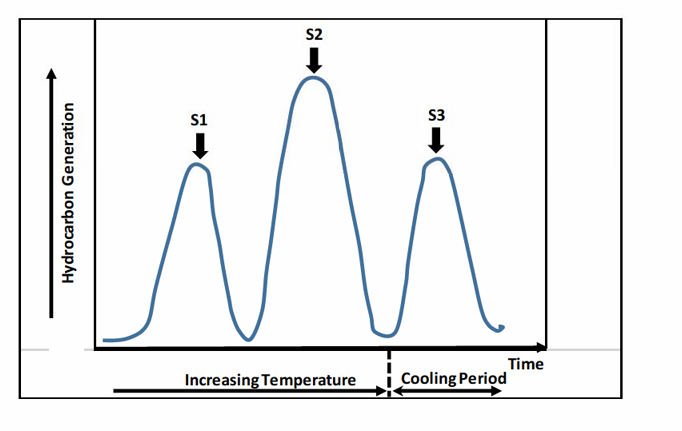
\includegraphics[width=0.5\linewidth]{figs/Q.33.png}
    \caption{fig7}
    \label{fig:figs/Q.33.png}
\end{figure}
\hfill{GATE 2019 PI}

\begin{multicols}{2}
\begin{enumerate}
    \item Peak S1 represents volatilization of existing hydrocarbons.
    \item Peak S2 represents breakdown of kerogen and generation of hydrocarbons.
    \item Peak S3 represents $T_{\text{max}}$, the temperature at which most hydrocarbons are generated.
    \item S1/(S1+S2) represents the production index.
\end{enumerate}
\end{multicols}
\item A single well encounters multiple clean sands of exactly the same thickness, porosity and permeability. $R_w$ is the formation fluid resistivity and $R_{mf}$ is the mud filtrate resistivity.

\begin{tabular}{ll}
P. $R_{mf} > R_w$ & I. No deflection \\
Q. $R_{mf} = R_w$ & II. Positive deflection \\
R. $R_{mf} < R_w$ & III. Negative deflection \\
\end{tabular}

Which one of the following match the relation between $R_w$ and $R_{mf}$ to that of Self Potential (SP) log deflection?

\hfill{GATE 2019 PI}

\begin{multicols}{2}
\begin{enumerate}
    \item P-I, Q-III, R-II
    \item P-III, Q-I, R-II
    \item P-II, Q-I, R-III
    \item P-I, Q-II, R-III
\end{enumerate}
\end{multicols}

\item Which one of the following options is NOT a part of the mudlogs prepared by the drill-site geologist?

\hfill{GATE 2019 PI}

\begin{multicols}{2}
\begin{enumerate}
    \item Rate of Penetration (ROP)
    \item Chromatograph showing presence of C$_1$ to C$_5$ concentration
    \item Lithology from drill cutting and its interpretation
    \item Reservoir unit delineation based on volume of shale ($V_{sh}$)
\end{enumerate}
\end{multicols}
\item Match the following:

\begin{tabular}{ll}
P. Location of storing the kelly on the trip & I. Mousehole \\
Q. Location of storing the next drill pipe    & II. Rathole \\
R. Location of storing pump pressure gauges   & III. Top drive \\
S. Rotational system that controls a drill string without a kelly & IV. Standpipe \\
\end{tabular}

\hfill{GATE 2019 PI}

\begin{multicols}{2}
\begin{enumerate}
    \item P-II, Q-I, R-IV, S-III
    \item P-IV, Q-II, R-III, S-I
    \item P-II, Q-I, R-III, S-IV
    \item P-IV, Q-III, R-II, S-I
\end{enumerate}
\end{multicols}

\item A box contains 2 red and 3 black balls. Three balls are randomly chosen from the box and are placed in a bag. Then the probability that there are 1 red and 2 black balls in the bag, is \rule{3cm}{0.15mm}.

\hfill{GATE 2019 PI}

\item The values of a function $f(x)$ over the interval $[0,4]$ are given in the table below:

\begin{center}
\begin{tabular}{|c|c|c|c|c|c|}
\hline
$x$      & 0   & 1   & 2   & 3   & 4    \\
\hline
$f(x)$   & 1   & 0.5 & 0.2 & 0.1 & 0.06 \\
\hline
\end{tabular}
\end{center}

Then, according to the trapezoidal rule, the value of the integral $\int_{0}^{4} f(x)\,dx$ is \rule{3cm}{0.15mm} (round off to 2 decimal places).

\hfill{GATE 2019 PI}
\item Oil is produced at a constant rate from a well in a bounded reservoir. The variation of the bottom-hole pressure with time is shown in the given Table. The \textbf{magnitude} of the slope of the pressure vs time curve that you would use to find the drainage area is \rule{2.5cm}{0.15mm} psi/day (round off to 1 decimal place).

\begin{center}
\begin{tabular}{|c|c|c|c|}
\hline
Time (days) & Flowing bottom- & Time (days) & Flowing bottom- \\
            & hole pressure (psi) &           & hole pressure (psi) \\
\hline
0 & 3500 & 6  & 2512 \\
1 & 2864 & 7  & 2482 \\
2 & 2725 & 8  & 2452 \\
3 & 2644 & 9  & 2422 \\
4 & 2587 & 10 & 2392 \\
5 & 2542 & 11 & 2362 \\
\hline
\end{tabular}
\end{center}

\hfill{GATE 2019 PI}

\item In a core flood experiment of immiscible and incompressible displacement of oil ($\mu_o = 1$ cP) with water ($\mu_w = 1$ cP), only axial flow is observed. The relative permeability of water is given by $k_{rw} = S_w^2$, where $S_w$ is water saturation. The relative permeability of oil is given by $k_{ro} = (1-S_w)^2$. The gravity and capillary pressure are neglected. From the fractional flow and water saturation relationship, the saturation of water at the flood front is \rule{2.5cm}{0.15mm} \% (round off to 1 decimal place).

\hfill{GATE 2019 PI}

\item In an oil well, the pressure at the gas oil contact (GOC) at a depth of 2000 m is 205 bar (gauge), as shown in the figure.
\begin{figure}[H]
    \centering
    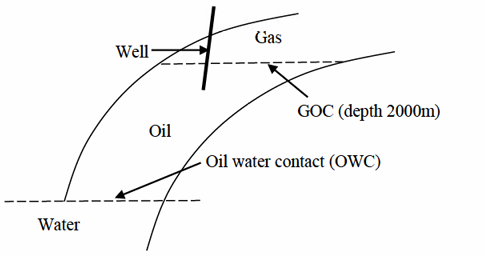
\includegraphics[width=0.5\linewidth]{figs/Q.41.png}
    \caption{fig8}
    \label{fig:figs/Q.41.png}
\end{figure}
The static oil pressure gradient is 0.08~bar/m in the pay zone. If a constant hydrostatic pressure gradient of 0.1~bar/m prevails throughout the subsurface, then the thickness of the oil column is \rule{2cm}{0.15mm}~m (round off to 1 decimal place).
\hfill{GATE 2019 PI}
\item Oil is produced at a constant rate of $10 \ \mathrm{m^3/day}$ from a reservoir for 500 days. The producing gas oil ratio (GOR) is constant at $10 \dfrac{m^3_{gas}}{m^3_{oil}}$ for the first 100 days. Then, the producing gas oil ratio increases linearly and on the 500$^{th}$ day the measured GOR is $50 \dfrac{m^3_{gas}}{m^3_{oil}}$. The cumulative produced gas oil ratio after 500 days of production is \rule{2cm}{0.15mm} $\dfrac{m^3_{gas}}{m^3_{oil}}$ (round off to 1 decimal place). Assume that all volumes are measured at STP.

\hfill{GATE 2019 PI}

\item A pressure build-up test was conducted in a well after 1000 days of producing oil at a constant rate of 0.01 reservoir-$\mathrm{m^3/s}$. The two shut-in bottom-hole pressure readings taken at 0.5 day and 1 day after shut-in are $150 \times 10^5$ Pa and $151 \times 10^5$ Pa, respectively. These pressure points correspond to the linear region of the Horner's plot. The reservoir thickness is 100 m and oil viscosity is 0.001 Pa$\cdot$s. The permeability of the reservoir is \rule{2cm}{0.15mm} mD (round off to 1 decimal place). [1 mD $= 10^{-15}~\mathrm{m^2}$].

\hfill{GATE 2019 PI}

\item In an oil reservoir, the residual oil saturation in the volume flooded with polymer solution is 20\%. The initial water saturation is 20\%. The volumetric sweep efficiency is 50\%. The maximum possible recovery factor for the reservoir is \rule{2cm}{0.15mm} \% (round off to 1 decimal place).

\hfill{GATE 2019 PI}
\item An electrical submersible pump (ESP) delivers well fluid with 100\% watercut. In the ESP, the impeller diameter is 0.1~m and speed is 3600~rpm. The total head developed by the ESP is 300~m (water column height). If the stage efficiency of the ESP is 60\%, then the minimum number of stages required is \rule{2cm}{0.15mm}~ (round off to nearest integer). [$g = 9.81~\mathrm{m/s}^2$]

\hfill{GATE 2019 PI}

\item In a counter flow heat exchanger, hot fluid enters at $100^\circ$C and leaves at $50^\circ$C. Cold fluid enters at $30^\circ$C and leaves at $40^\circ$C. If heat losses are ignored, then the logarithmic mean temperature difference (LMTD) is \rule{2cm}{0.15mm}~$^\circ$C (round off to 1 decimal place).

\hfill{GATE 2019 PI}

\item A model porous block of cross sectional area ($A$) and length ($L$) is made up of $N$ independent capillaries of equal radii ($r$) and length ($L$). The porosity of the block is 10\%, and the permeability for a laminar, incompressible and steady state flow is 0.02~mD. If the flow is only through the capillaries, then the value of $r$ is \rule{2cm}{0.15mm}~$\times~10^{-6}$~cm (round off to 1 decimal place). [1~mD~$= 10^{-15}$~m$^2$].

\hfill{GATE 2019 PI}

\item A model porous medium of 5 cylindrical capillaries of radii varying from 60 to 100 micrometers (refer Table) is subjected to Mercury Injection Capillary Pressure (MICP) treatment. The capillaries are being filled in an increasing order of their entry pressure. The magnitude of $(\sigma\cos\theta)_{air-Hg}$ is $367~\dfrac{\text{dyne}}{\text{cm}}$, where $\sigma$ is the interfacial tension and $\theta$ is the contact angle. The minimum applied mercury pressure to achieve 50\% mercury saturation in the sample is \rule{2cm}{0.15mm}~$\times~10^3$~dyne/cm$^2$ (round off to 1 decimal place).

\begin{center}
\begin{tabular}{|c|c|c|c|}
\hline
Radius & Cross- sectional & Cross-sectional Area & Cumulative Area \\
($\mu$m) & Area ($\mu$m$^2$) & (fraction) & (fraction) \\
\hline
60 & 11304 & 0.11 & 1.00 \\
70 & 15386 & 0.15 & 0.89 \\
80 & 20096 & 0.19 & 0.74 \\
90 & 25434 & 0.25 & 0.55 \\
100 & 31400 & 0.30 & 0.30 \\
\hline
\multicolumn{1}{c}{Total Area =} & \textbf{103620} & & \\
\end{tabular}
\end{center}

\hfill{GATE 2019 PI}
\item The sonic log parameters from an exploratory well in a reservoir are as follows: \\
Measured P-wave transit time ($\Delta t_{log}$) = 85~$\mu$s/ft \\
True resistivity ($R_t$) = 10~ohm-m \\
Matrix transit time ($\Delta t_{ma}$) = 45~$\mu$s/ft \\
Fluid transit time ($\Delta t_{fl}$) = 205~$\mu$s/ft \\
Formation water resistivity at reservoir temperature ($R_w$) = 0.1~ohm-m

The hydrocarbon saturation (in percentage) in the reservoir is \rule{2cm}{0.15mm}~(round off to 1 decimal place).

[Hint: Wyllie time average equation is $\Delta t_{log} = (1-\phi)\Delta t_{ma} + \phi \Delta t_{fl}$ and formation water resistivity has the correlation $R_w = \frac{1}{a} \phi^2 R_t S_w^2$, where $S_w$ is water saturation, $\phi$ is porosity and $a=1$ ]
\hfill{GATE 2019 PI}
\item A vertical well of 8000~ft is producing below bubble point pressure. Oil and water each is produced at the rate of 500~bbl/day. The indicated bottom hole pressure is 3000~psi. If the same gas to liquid ratio (GLR) is maintained, using the given figure, the new bottom hole pressure at 5000~ft is \rule{2.5cm}{0.15mm}~psi.
\begin{figure}[H]
    \centering
    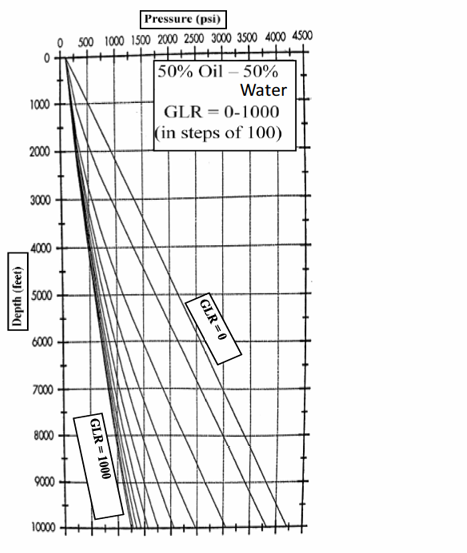
\includegraphics[width=0.5\linewidth]{figs/Q.50.png}
    \caption{fig9}
    \label{fig:figs/Q.50.png}
\end{figure}
\hfill{GATE 2007 PI}
\item In a drilling rig, the crown block and the traveling block have three and two sheaves, respectively. A single wireline connects the hoisting drum to the deadline anchor as shown in the figure. Neglect the weight of the pulleys and the wireline, and friction between the sheaves and wireline. The ratio of the deadline load to static crown load is \rule{2cm}{0.15mm}~(round off to 2 decimal places).

\begin{figure}[H]
    \centering
    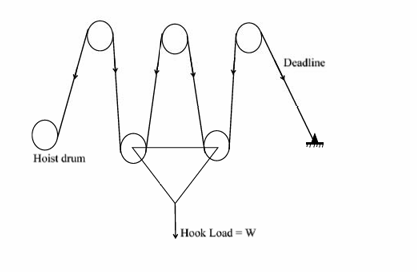
\includegraphics[width=0.5\linewidth]{figs/Q.51.png}
    \caption{fig10}
    \label{fig:figs/Q.51.png}
\end{figure}
\hfill{GATE 2019 PI}
\item Cement weighing 100~kg is mixed with 50~liters of water. The specific gravity of cement is 3.14 and the density of water is 1000~kg/m$^3$. Neglecting volume changes, the resulting density of the slurry is \rule{2cm}{0.15mm}~kg/m$^3$ (round off to 1 decimal place).

\hfill{GATE 2019 PI}

\item In an active water drive during a certain period, the rate of production and reservoir pressure remain constant. The water influx into the reservoir from the aquifer is 6000~bbl/day. The surface oil and water production rates are 3000~STB/day and 1500~STB/day, respectively. The current production gas to oil ratio is 825~SCF/STB, and the formation volume factors at the current pressure for oil, water and gas are 1.375~bbl/STB, 1.04~bbl/STB and 0.007~bbl/STB, respectively. The solution gas to oil ratio at the current pressure is \rule{2cm}{0.15mm}~SCF/STB (round off to 1 decimal place).

\hfill{GATE 2019 PI}

\item In a water flooding experiment, the pressure gradients in the displacing and displaced phases are 400~psi/ft and 350~psi/ft, respectively. Assume that the displacement front is stable in the absence of capillary and gravity forces. Consider that only water flows upstream and only oil flows downstream of the displacement front. Then the mobility ratio for this immiscible displacement process is \rule{2cm}{0.15mm}~(round off to 2 decimal places).

\hfill{GATE 2019 PI}
\item In a pressure draw-down testing, the well bore flowing pressure ($P_{wf}$) is given by
\[
P_{wf} = P_i - \frac{162.6\, q\, \mu\, B}{kh} \left[ \log\left( \frac{kt}{\phi \mu c r_w^2} \right) - 3.23 + 0.87 S \right].
\]
The following data is given in the oil field units, \\
Initial reservoir pressure ($P_i$) = 5000 psia \\
Pressure after 1 hr of production ($P_{1hr}$) = 4000 psia \\
Oil flow rate ($q$) = 500 STB/day \\
Porosity ($\phi$) = 0.25 \\
Viscosity of oil ($\mu$) = 2 cP \\
Formation volume factor of oil ($B$) = 1.2 bbl/STB \\
Formation thickness ($h$) = 20 ft \\
Total compressibility ($c$) = $30 \times 10^{-6}$ psi$^{-1}$ \\
Well bore radius ($r_w$) = 0.3 ft

The slope of $P_{wf}$ versus $\log t$ is $-100$ psi/cycle. Then, the skin factor ($S$) for this well is \rule{2cm}{0.15mm} (round off to 1 decimal place).

\hfill{GATE 2019 PI}

\end{enumerate}

\end{document}




















































    

















































































































\end{document}